%%!TEX encoding = UTF-8 Unicode

% According to UA rules, font size should range from 10 to 12pt.
\documentclass[12pt,a4paper,openright,final,twoside,onecolumn]{memoir}

\listfiles
\fixpdflayout

\usepackage[utf8]{inputenc}

% Computer Modern Typewritter (For bold ttfamily in listings)
\usepackage{lmodern}
% OR... Bera Mono
%\usepackage[scaled]{beramono} % TTT Font
%\usepackage{anyfontsize} % As the name says...

\usepackage[T1]{fontenc}

% For Overleaf support
\usepackage{ifthen}
\def\useoverleaf{0}  % change to non-zero (for instance, 1) to enable it

\makeatletter
\newcommand{\makecoverfile}[0]{%
  \immediate\write18{latexmk -pdf cover.tex}%
}
\makeatother

%For PDF merging
\usepackage{pdfpages}

%SET DPI to 300
\pdfpxdimen=\dimexpr 1in/300\relax

\usepackage{morewrites} % Allow the use of a larger number of packages

%For English and Portuguese languages
%Portuguese will be the default.
%Use \setdefaultlanguage to change it
\usepackage{csquotes}
\usepackage[portuguese,english]{babel}


% For custom date format
\usepackage{datetime}
\newdateformat{thesisdate}{\monthname[\THEMONTH] \THEYEAR} % Month Year

\usepackage{microtype} % Make pdf look better


% Uncomment to enable floats on facing pages
%\usepackage{dpfloat}

%Side by side figures
% Eg. Fig 1a, Fig 1b
\usepackage[hang,small,bf]{caption}
%\let\tion\undefined
%\let\subfloat\undefined
\usepackage{subcaption}

%\RequirePackage{textcase}

% Dropped Caps
%\usepackage{lettrine}

% Configure Hyperlink color
%\usepackage[breaklinks=true,colorlinks=false,linkcolor=blue]{hyperref}
% Or use the default
\usepackage{hyperref}

%Optional: Redefine section names
%\def\sectionautorefname{Section}
%\def\chapterautorefname{Chapter}
%\def\figureautorefname{Figure}
%\def\listingautorefname{Listing}
%\def\tableautorefname{Table}

%For PDF Comments
\usepackage{comment}
\usepackage{pdfcomment}
\usepackage{bookmark} % New Bookmarks

%For Multiple columns in Glossary
\usepackage{multicol}

%Math symbols
\usepackage{mathtools}
\usepackage{amsmath}
\usepackage{amssymb}
\DeclareMathOperator*{\argmax}{arg\,max}
\DeclareMathOperator*{\argmin}{arg\,min}
\DeclareMathOperator*{\mode}{mode}

%Graphics
\usepackage{graphicx}

%Colors
\usepackage{xcolor}

%Euro symbol
\usepackage{eurosym}

% Code boxes
\ifthenelse{\equal{\useoverleaf}{0}}
{\usepackage[outputdir=build]{minted}}
{\usepackage{minted}}%

%\renewcommand\listingscaption{Código}
\fvset{fontsize=\footnotesize} % Make Code blocks smaller than text

%Biber using IEEE style for proper UTF-8 support
\usepackage[backend=biber,style=ieee, sorting=none]{biblatex}
\bibliography{bib/references.bib, bib/rfc.bib}

%Use acronyms
\usepackage[printonlyused]{acronym} % For acronyms

% Enable chart support through pgf and tikz
\usepackage[version=0.96]{pgf}
\usepackage{tikz}
\usepackage{pgf-umlsd}
\usetikzlibrary{arrows,shadows,trees,shapes,snakes,automata,backgrounds,petri,mindmap} % for pgf-umlsd

%For Electric Circuits
\usepackage[detect-weight=true, binary-units=true]{siunitx}
\sisetup{load-configurations = binary}

\usepackage[american,cuteinductors,smartlabels]{circuitikz}

\usetikzlibrary{calc}
\ctikzset{bipoles/thickness=1}
\ctikzset{bipoles/length=0.8cm}
\ctikzset{bipoles/diode/height=.375}
\ctikzset{bipoles/diode/width=.3}
\ctikzset{tripoles/thyristor/height=.8}
\ctikzset{tripoles/thyristor/width=1}
\ctikzset{bipoles/vsourceam/height/.initial=.7}
\ctikzset{bipoles/vsourceam/width/.initial=.7}
\tikzstyle{every node}=[font=\small]
\tikzstyle{every path}=[line width=0.8pt,line cap=round,line join=round]

% For inline TT text (e.g. code snippets)
\usepackage{verbatim}

 %Frames around figures and allow force placement
\usepackage{float}

%Configure Float style
%\floatstyle{boxed}
%\restylefloat{table}
%\restylefloat{figure}
%\restylefloat{lstlisting}

%For test purposes
\usepackage{lipsum}

%Keep floats inside section!
\usepackage[section]{placeins}
\let \oldsubsubsection \subsubsection
\renewcommand{\subsubsection}[2][]{
  \FloatBarrier
  \oldsubsubsection#1{#2}
}
\let \oldsubsection \subsection
\renewcommand{\subsection}[2][]{
  \FloatBarrier
  \oldsubsection#1{#2}
}
\let \oldsection \section
\renewcommand{\section}[2][]{
  \FloatBarrier
  \oldsection#1{#2}
}
\let \oldchapter \chapter
\renewcommand{\chapter}[2][]{
  \FloatBarrier
  \oldchapter#1{#2}
}


%%%% Use the built-in division styling
\headstyles{memman}

%%% ToC down to subsections
\settocdepth{subsection}

%%% Numbering down to subsections as well
\setsecnumdepth{subsection}

%%%% extra index for first lines
\makeindex[lines]

%Margins for University of Aveiro Thesis
\setlrmarginsandblock{3cm}{2.5cm}{*}
\setulmarginsandblock{3cm}{3cm}{*}
\checkandfixthelayout

%Or custom spacing
%\addtolength{\parskip}{0.5\baselineskip}
\linespread{1.5}

\begin{document}
\ifthenelse{\equal{\useoverleaf}{0}}{}{\makecoverfile{}}%
\includepdf[pages=-]{cover.pdf}

%
%Front matter

%Custom Chapter style named thesis
\makechapterstyle{thesis}{% Based on ell
  \chapterstyle{default}
  \renewcommand*{\chapnumfont}{\normalfont\sffamily}
  \renewcommand*{\chaptitlefont}{\normalfont\Huge\sffamily}
  \settowidth{\chapindent}{\chapnumfont 111}
  \renewcommand*{\chapterheadstart}{\begingroup
    \vspace*{\beforechapskip}%
    \begin{adjustwidth}{}{-\chapindent}%
    \hrulefill
    \smash{\rule{0.4pt}{15mm}}
    \end{adjustwidth}\endgroup}
  \renewcommand*{\printchaptername}{}
  \renewcommand*{\chapternamenum}{}
  \renewcommand*{\printchapternum}{%
    \begin{adjustwidth}{}{-\chapindent}
    \hfill
    \raisebox{10mm}[0pt][0pt]{\fontsize{30}{25}\selectfont\chapnumfont \thechapter}%
                              \hspace*{1em}
    \end{adjustwidth}\vspace*{-3.0\onelineskip}}
  \renewcommand*{\printchaptertitle}[1]{%
    \vskip\onelineskip
    \raggedleft {\chaptitlefont ##1}\par\nobreak\vskip 4\onelineskip}}


%Select chapter style from existing or select custom
%\chapterstyle{thesis} % Others: dowding, demo2, dash, chappell, brotherton, bianchi, ger, madsen, tatcher, veelo,indexes)
% thesis can also be used as defined previously
%

%If you feel adventurous you can also define all aspects of your theme
%Use either this input or the chapterstyle before
%% Rules
\newcommand{\thinRule}{\rule{\textwidth}{0.25pt}}

% Customize heading appearances
% Define styles
\newcommand{\partSize}{\Huge}
\newcommand{\partStyle}{\lsstyle\scshape}
\newcommand{\chapterSize}{\Huge}
\newcommand{\chapterStyle}{\lsstyle\scshape}
\newcommand{\chapterAfter}{}
\newcommand{\sectionSize}{\Large}
\newcommand{\sectionStyle}{\scshape\MakeTextLowercase}
\newcommand{\subsectionSize}{\large}
\newcommand{\subsectionStyle}{\scshape\MakeTextLowercase}
\newcommand{\subsubsectionSize}{\large}
\newcommand{\subsubsectionStyle}{\scshape\MakeTextLowercase}
\newlength{\partNumSizePt}
\setlength{\partNumSizePt}{60pt}
\newlength{\chapterNumSizePt}
\setlength{\chapterNumSizePt}{60pt}
\newcommand{\partNumSize}{%
  \fontsize{\partNumSizePt}{1.2\partNumSizePt}\selectfont%
}
\newcommand{\partNumStyle}{\partChapterNumColor}
\newcommand{\chapterNumSize}{%
  \fontsize{\chapterNumSizePt}{1.2\chapterNumSizePt}\selectfont%
}
\newcommand{\chapterNumStyle}{\partChapterNumColor}

% Customize parts
\renewcommand{\partnamefont}{\partSize\partStyle}
\renewcommand{\partnumfont}{\partNumSize\partNumStyle}
\renewcommand{\printpartname}{}
\renewcommand{\printparttitle}[1]{%
  \normalfont\normalcolor\partnamefont #1
}

% Customize chapters
\makeatletter
\setlength{\beforechapskip}{30pt}
\renewcommand*{\chapterheadstart}{\vspace*{\beforechapskip}}
\setlength{\afterchapskip}{3ex}
\setlength{\midchapskip}{3ex}
\renewcommand*{\chapnamefont}{%
  \Large\flushright\chapterStyle\partChapterNumColor%
}
\renewcommand*{\chapnumfont}{\chapterNumSize\chapterNumStyle}
\renewcommand*{\chaptitlefont}{%
  \normalfont\flushleft\normalcolor\chapterSize\chapterStyle%
}
\renewcommand*{\printchaptername}{%
  \chapnamefont\MakeTextLowercase{\@chapapp}%
}
\renewcommand*{\chapternamenum}{\quad}
\renewcommand*{\printchapternum}{%
%  \chapnumfont\textls[-75]{\classicstylenums{\thechapter}}%
 \chapnumfont\textls[-75]{\thechapter}%

}
\renewcommand*{\printchaptertitle}[1]{%
  \chaptitlefont #1
  \chapterAfter
}
\makeatother
% Customize sections and subsections
\setsecnumformat{\csname my#1\endcsname\quad}
\setsecheadstyle{\sectionSize\sectionStyle}
\newcommand{\mysection}{{\thesection}}
\setlength{\beforesecskip}{3em}


\setsubsecheadstyle{\subsectionSize\subsectionStyle}
\newcommand{\mysubsection}{{\normalfont\subsectionSize\thesubsection}}
\setlength{\beforesubsecskip}{3em}

\setsubsubsecheadstyle{\subsubsectionSize\subsubsectionStyle}
\newcommand{\mysubsubsection}{{\normalfont\subsubsectionSize\thesubsubsection}}
\setlength{\beforesubsubsecskip}{2em}

% Customize "Table of ..." appearance
% Customize headings
\newcommand{\renewPrintXTitle}[1]{%
  \renewcommand{#1}[1]{%
    \printchaptertitle{##1}%
  }%
}
\renewPrintXTitle{\printtoctitle}
\renewPrintXTitle{\printlottitle}
\renewPrintXTitle{\printloftitle}

% Customize ToC headings
\renewcommand{\cftpartfont}{\partChapterNumColor\partStyle}
\renewcommand{\cftchapterfont}{\chapterStyle}
\renewcommand{\cftsectionfont}{}
\renewcommand{\cftsubsectionfont}{}
\renewcommand{\cftfigurefont}{}
\renewcommand{\cfttablefont}{}
\newcommand{\cftlstlistingfont}{}

% Increase number width
\newlength{\cftNumWidthIncrease}
\setlength{\cftNumWidthIncrease}{0.25em}
\addtolength{\cftpartnumwidth}{\cftNumWidthIncrease}
\addtolength{\cftchapternumwidth}{\cftNumWidthIncrease}
\addtolength{\cftsectionindent}{\cftNumWidthIncrease}
\addtolength{\cftsubsectionindent}{\cftNumWidthIncrease}
% No leader dots
%\renewcommand*{\cftpartdotsep}{\cftnodots}
%\renewcommand*{\cftchapterdotsep}{\cftnodots}
%\renewcommand*{\cftsectiondotsep}{\cftnodots}
%\renewcommand*{\cftsubsectiondotsep}{\cftnodots}
%\renewcommand*{\cftfiguredotsep}{\cftnodots}
%\renewcommand*{\cfttabledotsep}{\cftnodots}
%\newcommand*{\cftlstlistingdotsep}{\cftnodots}
% Set page numbers immediately after entry text
\newcommand{\tocEntryPageSep}{\hspace{1em}}
\renewcommand{\cftpartleader}{\cftdotfill{\cftdotsep}}
%\renewcommand{\cftpartafterpnum}{\cftparfillskip}
%\renewcommand{\cftchapterleader}{\tocEntryPageSep}
\renewcommand{\cftchapterleader}{\cftdotfill{\cftdotsep}}
%\renewcommand{\cftchapterafterpnum}{\cftparfillskip}
\renewcommand{\cftsectionleader}{\cftdotfill{\cftdotsep}}
%\renewcommand{\cftsectionafterpnum}{\cftparfillskip}
\renewcommand{\cftsubsectionleader}{\cftdotfill{\cftdotsep}}
%\renewcommand{\cftsubsectionafterpnum}{\cftparfillskip}
\renewcommand{\cftfigureleader}{\cftdotfill{\cftdotsep}}
%\renewcommand{\cftfigureafterpnum}{\cftparfillskip}
\renewcommand{\cfttableleader}{\cftdotfill{\cftdotsep}}
%\renewcommand{\cfttableafterpnum}{\cftparfillskip}
\newcommand{\cftlstlistingleader}{\cftdotfill{\cftdotsep}}
%\newcommand{\cftlstlistingafterpnum}{\cftparfillskip}
% Customize page numbers
\newcommand{\tocPageStyle}{\tocPageColor}
\renewcommand{\cftpartpagefont}{\tocPageStyle}
\renewcommand{\cftchapterpagefont}{\tocPageStyle}
\renewcommand{\cftsectionpagefont}{\tocPageStyle}
\renewcommand{\cftsubsectionpagefont}{\tocPageStyle}
\renewcommand{\cftfigurepagefont}{\tocPageStyle}
\renewcommand{\cfttablepagefont}{\tocPageStyle}
\newcommand{\cftlstlistingpagefont}{\tocPageStyle}

% Abstract
% Remove indents around abstract text
\setlength{\absleftindent}{0pt}
\setlength{\absrightindent}{0pt}
% Change font size to conform with the rest of the document text
\renewcommand{\abstracttextfont}{\normalsize}

% Customize headers and footers including page numbers
\newcommand{\hfTextSize}{\footnotesize}
\newcommand{\headTextStyle}{\lsstyle\scshape\MakeTextLowercase}
\nouppercaseheads
\makeevenhead{headings}%
             {\hfTextSize\thepage}%
             {}%
             {\hfTextSize\headTextStyle\leftmark}
\makeevenhead{plain}%
             {\hfTextSize\thepage}%
             {}%
             {\hfTextSize\headTextStyle\leftmark}
\makeoddhead{headings}%
            {\hfTextSize\headTextStyle\rightmark}%
            {}%
            {\hfTextSize\thepage}
\makeoddhead{plain}%
            {\hfTextSize\headTextStyle\rightmark}%
            {}%
            {\hfTextSize\thepage}


% Customize captions
\newcommand{\captionSize}{\small}
\newcommand{\captionStyle}{\scshape}
\newcommand{\captionWidthRatio}{0.9}

\captionnamefont{\captionSize\captionStyle}
\captiontitlefont{\captionSize}
\captiondelim{ -- }
\captiontitlefinal{}
\changecaptionwidth
%\captionwidth{\captionWidthRatio\textwidth}

% Define colors
%\newcommand{\titleColor}{\color[rgb]{0.616, 0.0627, 0.176}}
\newcommand{\titleColor}{\color[rgb]{0,0,0}}

\newcommand{\partChapterNumColor}{\titleColor}
\newcommand{\dropCapColor}{\titleColor}
%\newcommand{\tocPageColor}{\color[rgb]{0.0980, 0.329, 0.651}}

\newcommand{\tocPageColor}{\color[rgb]{0, 0,0}}
\definecolor{shade0}{rgb}{1.0 , 1.0 , 1.0 }
\definecolor{shade1}{rgb}{0.9 , 0.9 , 0.9 }
\definecolor{shade2}{rgb}{0.8 , 0.8 , 0.8 }
\definecolor{shade3}{rgb}{0.65, 0.65, 0.65}
\definecolor{shade4}{rgb}{0.45, 0.45, 0.45}
\definecolor{shade5}{rgb}{0.0 , 0.0 , 0.0 }



\chapterstyle{veelo}
%Exclude sub figures from List of Figures
%\captionsetup[subfloat]{list=no}


% Texts
\newenvironment{introduction}
{%
  \begin{minipage}{\textwidth}%
   \itshape%
}
{%
  \end{minipage}%
  \par\addvspace{2\baselineskip plus 0.2\baselineskip minus 0.2\baselineskip}%
}


%Select Page style
\pagestyle{plain}

\frontmatter

\tightlists
\midsloppy
\raggedbottom

\setcounter{tocdepth}{2} %subsections are added to the TOC
\setcounter{secnumdepth}{4} %subsubsections are numbered


\cleardoublepage

%Table of contents
{\small\tableofcontents}
\cleardoublepage

%List of figures
{\small\listoffigures}


%List of tables
\cleardoublepage
{\small\listoftables}

%Print Glossary
{\small\chapter{Glossary}

\footnotesize
\SingleSpacing

\begin{multicols}{2}
\begin{acronym}[AAAAAA]

	\acro{DL}[DL]{Deep Learning}
	\acro{ANN}[ANN]{Artificial Neural Network}
	\acro{CNN}[CNN]{Convolutional Neural Network}
	\acro{GPU}[GPU]{Graphics Processing Unit}
	\acro{CPU}[CPU]{Central Processing Unit}
	\acro{SGD}[SGD]{Stochastic Gradient Descent}
	\acro{PRNG}[PRNG]{Pseudo Random Number Generator}

\end{acronym}
\end{multicols}
}

%
%Main document starts here
%
\mainmatter



% Start of Thesis text ----------------------------------------------------------
%Line spacing: 1.5 pt
\OnehalfSpacing

\chapter{Introduction}
\label{chapter:introduction}

This introductory chapter introduces this dissertation's motivation, objectives, and high-level outline.

\section{Motivation}

Melanoma is a cancer that is developed from melanocytes, i.e. cells that produce the melanin skin pigment. This abnormal growth of tissue generally occurs in skin, but can also manifest itself in the mouth, intestines or eyes. The most common cause of melanoma is the exposure to ultraviolet light (e.g. sunlight, tanning devices), thus it can be prevented by frequent use of sunscreen and avoiding long exposure to the sun. The clinical diagnosis is confirmed with a skin biopsy and, if it hasn't spread, treatment is usually surgical excision.

Melanoma is a dangerous type of skin cancer which, in 2012, occurred in 232000 people, and in 2015 there were 3.1 million people with the disease that resulted in over 59000 deaths worldwide. According to the \ac{CDC} , the rates of new melanomas have doubled over the last three decades and will continue to double.

Since the skin lesions occur on the surface of the skin, melanoma can easily be detected early through visual inspection by a physician with the use of dermoscopy techniques that allow a better look at the pigmented lesions. Dermoscopy is an imaging technique that works by removing the surface reflection of the skin which enables the visualization of enhanced levels of skin. More recently, computerized digital dermoscopy has made it relatively trivial to get high resolution imaging that can be used to get second opinions remotely or even a computer-assisted diagnosis\cite{dermoscopy}. More specifically, advances in deep learning algorithms and computer hardware has made classification by a machine learning algorithm a viable and reliable technique for a diagnosis.

Deep learning architectures are an improvement of \ac{ANN} characterized by the large number of hidden processing layers capable of learning hierarchical feature representations. One major advantage of deep learning is that it reduces the need of feature engineering, which is one of the most complicated and time consuming parts in machine learning practice. The successes of deep learning architectures are now well reported in computer vision. The latest developments have been boosted by the use of \ac{GPU} to speedup computations and the development of high-level modules to build neural networks such as Theano, Caffe and TensorFlow.

The surveys by Greenspan, Ginneken and Summers \cite{intro1}, Hu et al. \cite{intro2} and Litjens et al. \cite{intro3} contribute to a clear understanding of the principles and methods of neural networks and deep learning applied to medical image analysis. They provide insight into how the algorithms based on deep models, namely \ac{CNN}, are being applied in different contexts, such as organ segmentation, lesion detection or tumor classification. A particular area where deep learning is rapidly improving the state-of-the art is in dermatology care \cite{nature2017}\cite{intro5}\cite{intro6}. The results achieved are impressive despite the many challenges for training deep models with many layers composed by adaptive parameters encompass.

The first challenge is that deep learning models often require a large amount of training data to achieve superior performance than other methods (shallow competitors). Second, the objective function is often a highly non-convex function of the parameters with the potential for local minima. Third, we still lack the right methodology to fully comprehend the deep structure of a trained model that works, to a large extent, like a black box. Consequently, training deep models from scratch requires large amounts of annotated data and massive computational resources. Transfer learning has emerged as a promising solution to the data challenge by using, as baseline, the knowledge from a deep model previously trained on a large labelled dataset \cite{intro7}\cite{howtransferable}\cite{intro9}.

\section{Objectives}

The objective is to assess and compare the effectiveness of transfer learning in the specific domain of skin lesion classification by running experiments that will train and evaluate models using various different techniques.

The first set of experiments focuses on transfer learning. In general, we start from models previously trained on ImageNet (of a variety of architectures) and repurpose them for the task of skin lesion classification by extracting weights from arbitrary layers and continuing training on our dataset. Namely in our study we consider as a variable the layer where this extraction of weights occurs and study its effect.

The second set of experiments focuses on a simpler custom \ac{CNN} architecture designed around first-principle heuristics and trained end-to-end, rather than the transfer learning approach of initializing the weights to those of the pre-trained model, thus presenting a model obtained by following more traditional techniques for comparison.

\section{Outline}

At a high level, this dissertation is organized into 5 other chapters:

\begin{itemize}
    \item Chapter \ref{chapter:background} introduces the reader to deep learning concepts and state-of-the-art techniques relevant to this dissertation;
    \item Chapter \ref{chapter:sota} reviews the state-of-the-art results of deep learning applied to dermoscopy;
    \item Chapter \ref{chapter:environment} introduces the hardware and software used for this work;
    \item Chapter \ref{chapter:experiments} goes over this work's methodology and presents and discusses the experimental results;
    \item Chapter \ref{chapter:conclusion} offers final remarks, key takeaways, and points in the direction of future work.
\end{itemize}

\chapter{State of the Art}
\label{chapter:sota}

This chapter reviews current state-of-the-art results in skin lesion classification and medical image analysis in general to get an overview of the work related to this dissertation and to establish a baseline for comparison.

\section{Transfer Learning Approaches}

\citeauthor{Brinker2018} \cite{Brinker2018} present the first systematic review of the cutting edge in lesion classification with deep convolutional neural networks, which remains the fundamental technique in state-of-the-art results. They review 13 papers that use \ac{CNN}, most of which transfer weights from networks trained on \ac{ILSVRC} to the target task, which speeds up training and reduces costs by leveraging previous knowledge. In conclusion they note that \ac{CNN} are currently the state-of-the-art in skin lesion classification and that transfer learning is a very effective approach, but that it was rather difficult to compare results given the heterogeneity of datasets (some of which are not public) making reproduceability difficult. This motivated the initiative by the ISIC Archive to collect and uniformize data as well as organize challenges to push new results.

In \citeyear{nature2017} \citeauthor{nature2017} \cite{nature2017} achieved perhaps the most famous result in skin lesion classification using deep learning, making it to the Nature scientific journal. Their dataset combines biopsy-proven data from the ISIC Archive, Edinburgh Dermofit Library, and the Stanford Hospital, totalling an astonishing 129450 samples (after going through data augmentation of random flips, rotations, crops) which remains one of the biggest efforts in data collection in the area. They build an undirected graph connecting images that were deemed to be similar and made sure that the connected components of this graph were separated and distributed between the train, validation, and test sets in order to create a more effective and diverse split of the data. The authors follow a transfer learning approach by leveraging the weights of the InceptionV3 network trained on ImageNet, on top of which they build their own classifier and fine-tune previous layers carefully using the RMSProp optimizer. They evaluate the performance of the network by pitting it against 21 board-certified dermatologists on biopsy-proven medically-relevant cases of keratinocyte carcinomas versus benign seborrheic keratoses and malignant melanomas versus benign nevi, attaining performance on par with experts.

\citeauthor{menegola2017} \cite{menegola2017} went back to the ISIC 2016 lesion classification challenge to try to obtain better results and employed a transfer learning approach to leverage weights from VGG-16 and VGG-M networks originally trained on ImageNet and fine-tune the network on a dataset comprised of data from the ISIC 2016 challenge and the Interactive Atlas of Dermoscopy (augmented by randomly scaling, rotating or flipping the samples) which they train for 60 epochs using \ac{SGD} with momentum and L2 regularization to obtain a set of features on top of which they train an SVM classifier. They report results on the test set of the ISIC 2016 challenge, achieving 0.807 AUC with the deeper VGG-16 model. Their results further show that in really difficult cases their model is not very confident in its prediction, which suggests that, for the time being, current technology is better used as a reference to support and explain the diagnosis human doctors' rather than as a complete diagnosis framework.

\subsection{ISIC 2017 Part 3: Lesion Classification}

In part 3 of the ISIC 2017 \cite{isic2017} challenge participants were asked to develop two binary classifiers to distinguish between:

\begin{itemize}
    \item melanoma vs nevus and seborrheic keratosis
    \item seborrheic keratosis vs nevus and melanoma
\end{itemize}

Participants were given a training set of 2000 images (374 melanoma, 254 seborrheic keratosis, and the remaining 1372 benign nevi), a validation set of 150 images and a test set of 600 images. The images were of questionable quality and required a lot of preprocessing effort, which they could also complement by gathering their own data. Participants were ranked and awarded based only on AUC, but other metrics were reported for scientific completeness.

% first place
First place was a joint effort between Casio and Shinshu University presented by Kazuhisa Matsunaga et al\cite{isic2017first}. In their work they adopted ensembles of their own variant of ResNet-50 that they trained presumably end-to-end (using RMSProp\cite{rmsprop} and AdaGrad\cite{adagrad}) on data from the challenge as well as data they gathered independently, which was normalized in such a way to exploit color constancy and of which multiple geometric transformations were input in parallel to the networks.

The metadata available in the training set showed that melanoma and seborrheic keratosis were both uncommon in young ages. From this observation they implemented a simple thresholding by age, which improved performance for seborrheic keratosis classification from 0.957 to 0.960 AUC in cross-validation but not for melanoma classification. They noted that a more careful thresholding implementation is necessary from a clinical point of view. In the end, the mean performance of the two classifiers on the validation set was 0.958 AUC and, after the paper was published, 0.911 on the test set.

% second place
Iván from the Universidad Carlos III de Madrid \cite{isic2017second} got second place by designing a very complete automatic diagnosis system where a dermoscopic image goes through:

\begin{enumerate}
    \item A segmentation network based on \ac{FCN} \cite{fcn} to generate a binary mask outlining the area actually occupied by the lesion
    \item A data augmentation module to generate random label-invariant views of the original dermoscopic image through rotations and crops.
    \item A structure segmentation network that produces binary masks for 8 heuristically designed structures (dots, reticular patterns and pigmented networks, homogeneous areas, regression areas, blue-white veil, streaks, vascular structures, and other unspecific patterns) that expert dermatologists find important for a diagnosis
    \item A classification network based on transfer learning from ResNet-50 \cite{resnet} that takes into consideration the structures identified by the structure segmentation network as well as the original dermoscopic image.
\end{enumerate}

This effort resulted in AUC score of 0.910 on the test set, thus earning second place.

% third place
Third place was an effort by Afonso Menegola et al \cite{isic2017third} from RECOD Lab. who collected several datasets which they cleaned and filtered, resulting in two sets of 9640 and 7544 images with differing performances on the two different binary classification tasks that they decided to keep in consideration throughout their experiments. They adopted a transfer learning approach and decided to focus on ResNet-101 and Inception-V4 models trained on ImageNet on top of which they experimented with:

\begin{itemize}
    \item Curriculum learning scheme in which they schedule the samples during training such that easier samples are batched first and harder samples are batched later. However in practice this was worse than a traditional learning scheme.
    \item Training data and testing data augmentation by applying label-invariant random transformations such as crops, flips, etc. that ended up significantly improving performance (which the authors already knew from experience).
    \item Meta-learning scheme to take into consideration the decision of multiple models (even by simply averaging the output probabilities) gave the best results on the official validation AUC, even when compared to the single best model.
    \item Normalizing the inputs to Inception networks by subtracting the average pixel value significantly improved performance, but further dividing by the standard deviation gave worse results than baseline.
\end{itemize}

Their final submission was a meta model that combined seven models based on Inception and ResNet networks trained on distinct datasets which were then stacked in a meta-learning layer based on SVM. In the end they placed third by getting an AUC score of 0.908 on the test set.

% others
Also worth noting is

\begin{itemize}
    \item \citeauthor{isic2017li} \cite{isic2017li} who present novel multi-scale fully convolutional residual networks (based on FCRN-88 \cite{fcrn}) trained on datasets augmented differently (which empirically proved to offer better performance) whose outputs are interpolated to the original scale and summed up to yield what the authors call possibility maps which are further refined by taking into a consideration a distance map representing the importance of each pixel. For comparison they also ran experiments with AlexNet, VGG16, ResNet-50, ResNet-101, Inception-v3, but their custom network outperformed them all with an AUC score of 0.912 as evaluated on the ISIC 2017 dataset.
    \item \citeauthor{yang2017} \cite{yang2017} whose work propose a multi-task learning scheme where lesion segmentation and classification are solved simultaneously by constructing a model that builds feature maps using \ac{CNN} which then branches out into 3 parallel paths whose outputs individually do segmentation, melanoma binary classification, and seborrheic keratosis binary classification, but training is performed as if it was a single network optimizing parameters as usual. They achieve an AUC score of 0.926.
\end{itemize}

\subsection{ISIC 2018 Part 3: Lesion Classification}

In part 3 of the ISIC 2018 challenge participants were asked to develop a classifier to distinguish between:

\begin{itemize}
    \item Melanoma
    \item Melanocytic nevus
    \item Basal cell carcinoma
    \item Actinic keratosis
    \item Benign keratosis
    \item Dermatofibroma
    \item Vascular lesion
\end{itemize}

The provided training data comes from the HAM10000 Dataset \cite{ham10000}, which was acquired with many different dermatoscopes, from most anatomic sites, from a historical sample of patients presented for skin cancer screening, from many different institutions, with the proper approval. Diagnosis ground truth labels were established by:

\begin{itemize}
    \item Histopathology
    \item Reflectance confocal microscopy
    \item Lesion did not change during digital dermatoscopic follow up over two years with at least three images
    \item Consensus of at least three expert dermatologists from a single image
    \item Histopathology confirmation in cases of malignancy
\end{itemize}

Just like in the 2017 edition, participants could, of course, complement the training data by gathering their own, but this time they were ranked based on normalized multi-class accuracy metric.

In the 2018 edition \citeauthor{isic2018first} \cite{isic2018first} won first, second, and third place, attaining, respectively, a balanced multiclass accuracy of 0.885, 0.882, and 0.871 (which still beat fourth place by a margin of 2\%). In their work they combined data from the competition's HAM10000 dataset, the ISIC Archive, and other proprietary data, which were preprocessed using the Shades of Gray method to normalize images from different sources and contexts. Further in their data pipeline they augment training data by performing random horizontal flips, random rotations of ${0, 90, 180, 270}$ degrees, change brightness, saturation, and contrast by a random factor in the range $[0.9, 1.1]$. Their models were based on transfer learning from models trained on ImageNet like InceptionV3, ResNet-50, Squeezenet, Densenet, and others, of which they picked the best-performing and ensembled them in a stacking scheme.

The authors note that a large ensemble of models like theirs is not practical in production because of the high computational cost associated with infering the prediction of a given input for all models in the ensemble. For this reason, they suggest that constraints on memory usage or \ac{FLOPS} be considered in future challenges.

Noteworthy are also the submissions by

\begin{itemize}
    \item \citeauthor{isic2018milton} \cite{isic2018milton} who also followed an approach based on transfer learning from models of PNASNet-5-Large, InceptionResNetV2, SENet154, InceptionV4 trained on ImageNet, who interestingly noted that in the first few epochs the gradient is very erratic and thus refrained from fine-tuning weights during the first 2 epochs to avoid updating weights towards the wrong direction, in the end achieving a score of 0.76 on the validation set;
    \item \citeauthor{isic2018bissoto} \cite{isic2018bissoto} (who won 3rd place in the 2017 edition) which transfered knowledge from models of InceptionV4, ResNet-152, and DenseNet-161 trained on ImageNet, by training with online data augmentation (e.g. random crops, flips, rotations, shears, color transformations), \ac{SGD} with the learning rate being decreased by a factor of 10 whenever validation loss didn't improve for 10 epochs, eventually building an average of 15 models trained only with the challenge data that attained a score of 0.803.
\end{itemize}

\section{Hybrid Learning Techniques}

Clearly the large majority of the work in skin lesion classification follows a transfer learning approach, presumably because of how cost-effective it is (especially for smaller research teams). Nonetheless there has been some research that explore other techniques in addition to transfer learning.

\citeauthor{hybrid2} \cite{hybrid2} present an approach that extracts features from

\begin{itemize}
    \item a \ac{VGG} network originally trained on ImageNet
    \item unsupervised feature learning using sparse coding
\end{itemize}

and respectively trains two non-linear \ac{SVM} (using a histogram intersection kernel and sigmoid feature normalization) whose outputs are mapped to probabilities at a 50\% threshold and fused together using unweighted score averaging. They compare this against a more classical ensemble approach using only hand-coded low-level features, which used to be the state-of-the-art but is now significantly less performant at 0.715 accuracy on their test set (versus the 0.739 accuracy of the hybrid approach).

The work by \citeauthor{hybrid1} \cite{hybrid1} combines different techniques into a similar (but more extensive) classification framework that basically:

\begin{enumerate}
    \item extracts various features across two input scales (an area cropped around the segmented lesion, and the entire original dermoscopic image)
    \begin{itemize}
        \item hand-engineered rule-based features like color histogram, edge histogram, and color local binary patterns;
        \item unsupervised learning features from a sparse coded representation;
        \item features extracted from two deep residual networks trained on ImageNet and fine-tuned on the target dataset;
        \item the segmentation produced by their U-Net segmentation network is also used as a shape descriptor feature.
    \end{itemize}
    \item trains non-linear \ac{SVM} to learn a classifier for each extracted set of features;
    \item averages the output of each classifier in an ensemble to produce a final classification.
\end{enumerate}

When compared to an average of 8 dermatologists' predictions on 100 test images, they produce a higher accuracy and specificity evaluated at an equivalent sensitivity.

\chapter{Methodology}
\label{chapter:methodology}

This section describes, in detail, the methodology behind this dissertation's research objectives, namely:

\begin{itemize}
    \item Dataset description, preprocessing steps, and augmentation techniques;
    \item Software stack used to describe said experiments in code;
    \item Computational resources used to execute the experiments.
\end{itemize}

\section{Data}

The \ac{ISIC} 2017: Skin Lesion Analysis Towards Melanoma Detection grand challenge datasets \cite{isic2017} provides a training set with 2000 samples (divided into three classes: 374 melanoma, 254 seborrheic keratosis, and 1372 nevus), a validation set with 150 samples, and a test set with 600 samples. However training deep neural networks for skin lesion classification requires vast amounts of high quality, reliably labeled and verified data - a set of requirements which this dataset did not meet with confidence.

The \ac{HAM10000} \cite{ham10000} dataset is an effort to boost research on automated diagnosis of dermatoscopic images that focuses on the quality and reliability of the large volume of data that is so important for successful deep learning. The extracted images (where the lesion is centered if necessary) go through an extensive semi-automatic process that filters out non-dermoscopic imaging and unreliable diagnoses, after which they are submitted to a manual review to further confirm its quality.

The datasets from the \ac{ISIC} 2018 grand challenge \cite{isic2018} were largely based on \ac{HAM10000} that was already very high quality, which meant the data preprocessing needs would be much lower compared to the previous years' editions where all these quality guarantees had to be independently ensured by the competitors. The \ac{ISIC} 2018 datasets are therefore adequate for running these experiments.

\subsection{Preprocessing}
\label{subsection:preprocessing}

The images in the dataset undergo a number of preprocessing steps:

\begin{enumerate}
    \item Most readily available pretrained models are of network architectures whose input tensor is of square dimensions (e.g. $224 \times 224 \times 3$). Since our dataset's images are of distinct non-square dimensions, it is necessary to resize them to a square. However, resizing them all naively to the network's input tensor dimensions without regards to the image's aspect ratio means that the input fed to the network is of varying distinct aspect ratios which does not constitute a good start. Therefore, the first step is to crop an arbitrarily-sized square of the center of the image which will likely (and, in fact, does) capture the skin lesion.

    \begin{listing}[ht]
    \begin{minted}{python}
    def _crop(img):
        width, height = img.size
        if width == height:
            return img

        length = min(width, height)

        left = (width - length) // 2
        upper = (height - length) // 2
        right = left + length
        lower = upper + length

        box = (left, upper, right, lower)
        return img.crop(box)
    \end{minted}
    \caption{Function that crops a given image to a square crop of the center of the original image.}
    \label{code:crop}
    \end{listing}

\item Resize the images to the target networks' input dimensions $224 \times 224 \times 3$ and $299 \times 299 \times 3$. We resize (using nearest-neighbor interpolation) them as soon as possible in the data pipeline in order to reduce the computational costs of any subsequent operations on the images.

    \begin{listing}[ht]
    \begin{minted}{python}
    def _resize(img, target_size):
        return img.resize(target_size, PIL.Image.NEAREST)
    \end{minted}
    \caption{Function that resizes a given image to the target dimensions.}
    \label{code:resize}
    \end{listing}

    \item Normalize the luminance and apply a 99\% contrast stretch to reduce the negative effect of changes in illumination and acquisition devices that alter the color of images \cite{colorconstancy}.

    \begin{listing}[ht]
    \begin{minted}{python}
    def _correct(img):
        img_y, img_b, img_r = img.convert('YCbCr').split()

        img_y_np = np.asarray(img_y).astype(float)

        img_y_np /= 255
        img_y_np -= img_y_np.mean()
        img_y_np /= img_y_np.std()
        scale = np.max([np.abs(np.percentile(img_y_np, 1.0)),
                        np.abs(np.percentile(img_y_np, 99.0))])
        img_y_np = img_y_np / scale
        img_y_np = np.clip(img_y_np, -1.0, 1.0)
        img_y_np = (img_y_np + 1.0) / 2.0

        img_y_np = (img_y_np * 255 + 0.5).astype(np.uint8)

        img_y = PIL.Image.fromarray(img_y_np)

        img_ybr = PIL.Image.merge('YCbCr', (img_y, img_b, img_r))
        return img_ybr.convert('RGB')
    \end{minted}
    \caption{Function that normalizes the luminance of an image and applies a 99\% contrast stretch.}
    \label{code:correct}
    \end{listing}
\end{enumerate}

\subsection{Augmentation}
\label{subsection:augmentation}

In our binary classification task (melanoma vs non-melanoma) the $m = 10015$ samples in the training set are highly imbalanced (illustrated in figure \ref{fig:classimbalance}):

\begin{itemize}
    \item the majority class has $|S_{maj}| = 8902$ samples, constituting $\frac{8902}{10015} \times 100 = 88.9\%$ of the samples;
    \item the minority class has $|S_{min}| = 1113$ samples, constituting $\frac{1113}{10015} \times 100 = 11.1\%$ of the samples.
\end{itemize}

\begin{figure}[ht]
    \centering
    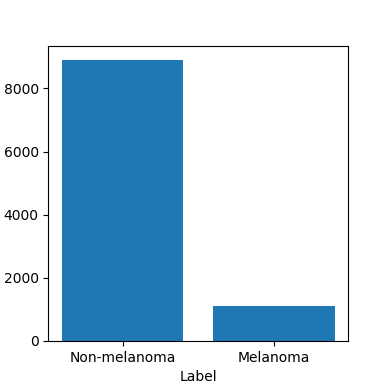
\includegraphics[width=0.5\textwidth]{figs/data_barplot.png}
    \caption{Bar plot of the distribution of the dataset's labels (melanoma or non-melanoma cases).}
    \label{fig:classimbalance}
\end{figure}

We correct this imbalance by oversampling the minority class, while also augmenting the total number of samples to $m' \approx 18000$ to increase the size of the dataset. That means we must augment the minority class by a factor of $\frac{\frac{m'}{2}}{|S_{min}|}$ and the majority class by a factor of $\frac{\frac{m'}{2}}{|S_{maj}|}$. For this augmentation we consider a set $T$ of possible transformations:

\begin{itemize}
    \item Horizontal flip
    \item Vertical flip
    \item 90º rotation
    \item 180º rotation
    \item 270º rotation
\end{itemize}

implemented by \verb|PIL.Image.transpose|\footnote{\url{https://pillow.readthedocs.io/en/stable/reference/Image.html\#PIL.Image.Image.transpose}} with the respective method:

\begin{itemize}
    \item \verb|PIL.Image.FLIP_LEFT_RIGHT|;
    \item \verb|PIL.Image.FLIP_TOP_BOTTOM|;
    \item \verb|PIL.Image.ROTATE_90|;
    \item \verb|PIL.Image.ROTATE_180|;
    \item \verb|PIL.Image.ROTATE_270|.
\end{itemize}

On principle, we did not consider transformations that change the color (e.g. contrast change, channel shift) or size (e.g. zoom) of features because it would unjustifiably allow the network to learn from these potentially misrepresenting features which even an expert human diagnosis would have trouble with.

The final available augmentations are all the $k$-combinations of the set $T$ for $k \in \{1, ..., |T|\}$, in other words all the possible ways in which you can combine the transformations from the set $T$.

\subsection{Split}

The number of variables in the future experiments would quickly lead to a combinatorial explosion of configurations, so to minimize the computational cost of the experiments a fixed validation scheme will be used rather than a cross validation scheme. To compensate for this lack of averaging over multiple folds of the data (which gives statistical confidence in the results), a fixed seed is set for every \ac{PRNG} as in code listing \ref{code:seed}, which in practice means parameters are initialized identically between experiments (providing some level of statistical confidence when making comparisons) and guarantees reproducibility.

\begin{listing}[ht]
\begin{minted}{python}
def seed():
    from random import seed
    seed(1)
    import numpy.random
    numpy.random.seed(2)
    from tensorflow import set_random_seed
    set_random_seed(3)
\end{minted}
\caption{Seed function that is called on every experiment to ensure reproducibility and similar conditions between experiments.}
\label{code:seed}
\end{listing}

The original training set from \ac{ISIC} 2018 is available for direct download, but the validation and test sets are kept private by the organization and are only used internally for reporting performance without actually releasing the data itself. As such, we will split the samples from the training set (which is available for download) into our own training, validation and test sets.

Augmentation, as described previously, results in 17810 samples which are split 85\%-15\% in a stratified fashion to maintain class balance within the splits into:

\begin{itemize}
    \item 15137 training samples, illustrated in figure \ref{fig:data_train};
    \item 2673 test samples, illustrated in figure \ref{fig:data_test}.
\end{itemize}

\begin{figure}[ht]
    \centering
    \includegraphics[width=0.6\textwidth]{../plots/data/train.png}
    \caption{Randomly-sampled images and respective labels of the train set.}
    \label{fig:data_train}
\end{figure}

\begin{figure}[ht]
    \centering
    \includegraphics[width=0.6\textwidth]{../plots/data/test.png}
    \caption{Randomly-sampled images and respective labels of the test set.}
    \label{fig:data_test}
\end{figure}

Since validation is intrinsically part of the training process itself, the validation set is a 15\% split from the training set obtained independently at the start of each training routine (also in a stratified fashion).

\section{Hardware}

Initially, computational resources from \ac{IEETA} were used in very early exploratory research:

\begin{itemize}
    \item Intel® Xeon® Processor E5-2640;
    \item NVIDIA Tesla K40c;
    \item NVIDIA Quadro K4000;
    \item 32GB DDR4 RAM.
\end{itemize}

However, given that it was shared between dozens of other researchers it was deemed not enough for a comfortable and flexible workflow because:

\begin{itemize}
    \item the little amount of memory almost wasn't enough to load the dataset into memory, especially during critically busy times;
    \item the NVIDIA Quadro K4000, with a compute capability of 3.0, was unsupported by the software stack which required a minimum compute capability of 3.7, leaving only a single NVIDIA Tesla K40c to work with.
\end{itemize}

More recently, \ac{LAR}, located in the Department of Mechanical Engineering at the University of Aveiro, has provided access to their deep learning research server codenamed Deeplar:

\begin{figure}[ht]
    \centering
    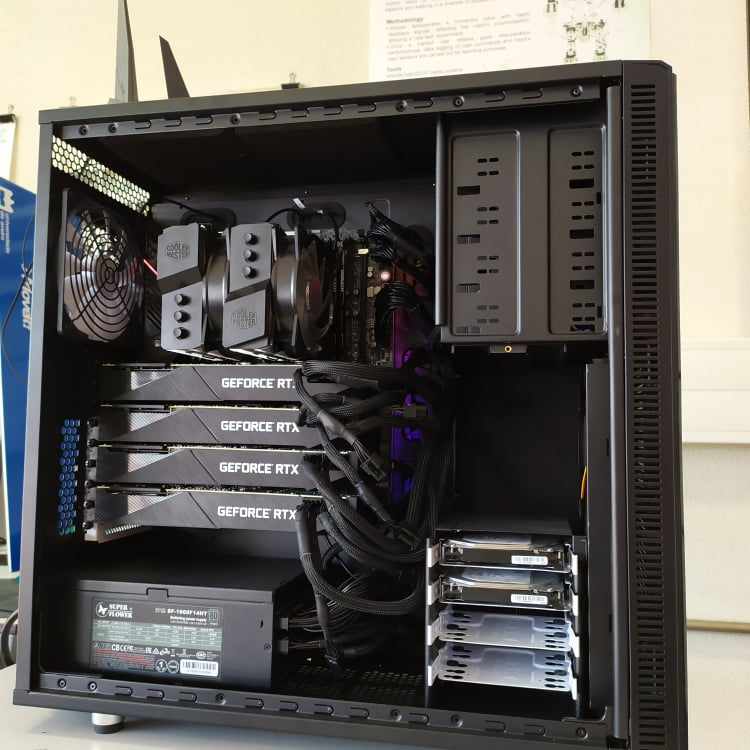
\includegraphics[width=0.4\textwidth]{figs/deeplar.jpg}
    \caption{Deeplar, the deep learning research server at \ac{LAR}}
    \label{fig:deeplar}
\end{figure}

\begin{itemize}
    \item AMD Ryzen™ Threadripper 2950X;
    \item Four NVIDIA GEFORCE® RTX 2080 Ti;
    \item 128GB DDR4 RAM.
\end{itemize}

The latter much more capable server (four state-of-the-art consumer \ac{GPU} and lots of \ac{RAM}) was effectively responsible for running this work's experiments.

\section{Software}

The deep learning research server Deeplar runs on openSUSE Tumbleweed 20191004\footnote{\url{https://software.opensuse.org/distributions/tumbleweed}}, a popular rolling-release GNU/Linux distribution. For interfacing with the \ac{GPU} it has installed CUDA 9.2 \footnote{\url{https://developer.nvidia.com/cuda-zone}} (NVIDIA GPU's proprietary language and API) and cuDNN 7.6.0 \footnote{\url{https://developer.nvidia.com/cudnn}} (a library for working with deep neural networks which most higher level frameworks rely on).

We used Miniconda\footnote{\url{https://docs.conda.io/en/latest/miniconda.html}} to install Conda\footnote{\url{https://conda.io/en/latest/}} which was used to manage a Python 3.6\footnote{\url{https://www.python.org/}} environment which was specifically required for compatibility with TensorFlow. Crucially, the following Python packages and specific versions were used for the development of most of the source code.

\begin{itemize}
    \item TensorFlow\footnote{\url{https://www.tensorflow.org/}} 1.12.0, of which we mostly use the \verb|tf.keras| API, for training and testing the various models;
    \item scikit-learn\footnote{\url{https://scikit-learn.org/}} 0.20.2 for some useful metrics and data splitting methods;
    \item NumPy\footnote{\url{https://numpy.org/}} 1.15.4 for various vector and matrix operations and Pillow\footnote{\url{https://pillow.readthedocs.io/en/stable/}} 5.4.1 for image handling and transformations because of this work's image preprocessing needs.
\end{itemize}

\chapter{Conclusion}
\label{chapter:conclusion}

In this section we present conclusions, final remarks, and point to directions for future work.

Ironically, when compared to end-to-end learning, most transfer learning experiments actually take longer because of the large number of parameters that you end up training anyway



% End of Thesis text ---------------------------------------------------------
% Including files is advised:


%Appendix

\backmatter


%Print all used references

\begingroup
\renewcommand{\bibfont}{\footnotesize}

%Redefine References name
\defbibheading{bibliography}[References]{
	\chapter{#1}
}
\SingleSpacing
\setlength\bibitemsep{8pt}
\printbibliography[heading=bibliography]
\endgroup


%Load appendix
%\include{appendix-a}


\end{document}
